\section{Auswertung}
\label{sec:Auswertung}

\subsection{Güteziffervergleich}
\begin{figure}
  \centering
  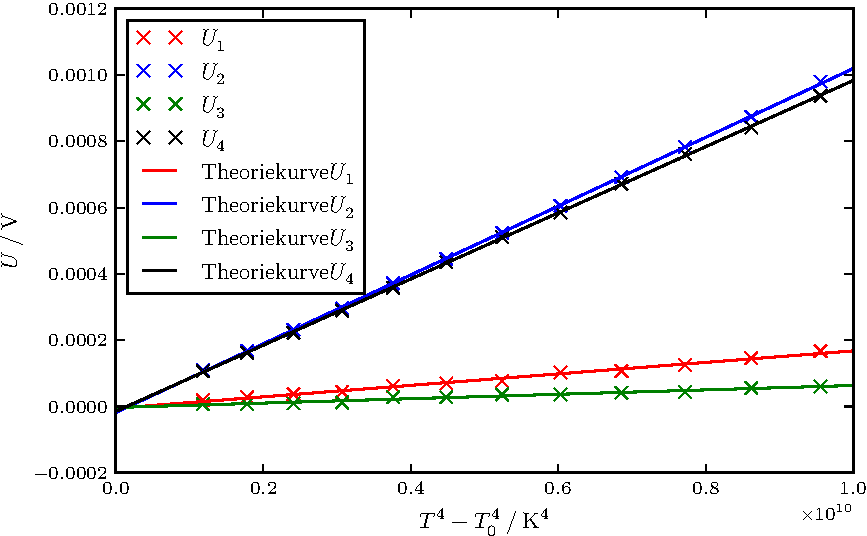
\includegraphics{plot.pdf}
  \caption{Plot.}
  \label{fig:plot}
\end{figure}
Die gemessenen Daten für die Tempeatur $T_1$ des wärmeren sowie die Temperatur
$T_2$ des kälteren Reservoirs wurden gegen die Zeit $t$ in Minuten abgetragen.
Mithilfe von SciPy wurde jeweils eine Ausgleichskurve für die folgende Funktion
berechnet:
\begin{equation}
  T(t)=A \cdot t^2 + B \cdot t + C
\end{equation}
Die Parameter $A$, $B$ und $C$ wurden bestimmt zu
\begin{align*}
A_{T_1} &= \SI{-3.87601 +- 0.10382e-6}{\kelvin\per\second²} \\
B_{T_1} &= \phantom{1}\SI{0.02345 +- 0.00019}{\kelvin\per\second} \\
C_{T_1} &= \phantom{1}\SI{293.592 +- 0.062}{\kelvin} \\
A_{T_2} &= \phantom{1}\SI{4.34879 +- 0.08533e-6}{\kelvin\per\second²}  \\
 B_{T_2} &= \SI{-0.01815 +- 0.00016}{\kelvin\per\second} \\
  C_{T_2} &= \phantom{1}\SI{294.936 +- 0.062}{\kelvin}
\end{align*}

Durch Ableiten und Einsetzen in die Ausgleichskurve
\begin{equation}
  \frac{\symup{d}T}{\symup{d}t}= 2 \cdot A \cdot t + B
\end{equation}
erhält man die Werte der Differentialquotienten. \\
Für eine ideale Wärmepumpe gilt
\begin{equation}
  v = \frac{T_1}{T_1-T_2}.
\end{equation}
Für die reale Wärmepunpe gilt jedoch die Formel
\begin{equation}
  v_{real}= \frac{\symup{d} Q_1}{\symup{d} tN} = (m_1c_w+m_kc_k)\frac{\symup{d} T_1}{\symup{d} tN}.
\end{equation}
wobei $ N = $ die Kompressorleistung, $ m_1$ die Masse des Wassers in $ R_1 $, $m_k$ die Masse des zu heizenden Reservoirs inklusive Kupferrohre, $ c_w $ die spezifische Wärmekapazität des Wassers sowie $ c_k $ die spezifische Wärmekapazität des Reservoirs und der Kuperrohre ist.
Da bei der Durchführung des Versuches \SI{4}{\litre} Wasser für $R_1$ verwendet wurden, berechnet sich $m_1$ zu $m_1 = \rho_{H_2O} \cdot V = \SI{4176.48}{\kilogram}$, wobei der Werte für $\rho_{H_20}$ der Literatur entnommen wurde.
Das Produkt aus $m_k$ und $c_k$ wurde vom Versuchsaufbau zu $\SI{750}{\joule\per\kelvin}$ abgelesen, $c_w$ wurde ebenfalls der Literatur zu $\SI{4,1819}{\kilo\joule\per\kilogram\kelvin}$ entnommen.
Die Kompressorleistung ergibt sich aus dem arithmetischen Mittelwert der Messdaten zu $N=124.77$.
Für die Differenzenquotienten wurden die Werte der Ausgleichskurve verwendet.
\begin{table}
  \centering
  \caption{Tabelle 1}
  \label{tab:tabelle1}
  \sisetup{table-format=1.2}
  \begin{tabular}{c c c c c c}
    \toprule
    {$t [\si{\second}]$} & {$T_1 [\si{\kelvin}]$} & {$T_2 [\si{\kelvin}]$} & {$\increment{T} [\si{\kelvin}]$} & {$\frac{\symup{d}T_1}{\symup{d}t}$} & {$\frac{\symup{d}T_2}{\symup{d}t}$}\\
    \midrule
    420 & 29.6 & 14.9 & 14.7 & 0.023397 & -0.01809 \\
    \bottomrule
  \end{tabular}
\end{table}
\subsection{Massendurchsatz}
